\documentclass[11pt, oneside]{article}
\usepackage[margin=1in]{geometry}
\geometry{letterpaper}
\usepackage[parfill]{parskip}
\usepackage{graphicx}
\usepackage{amssymb}
\usepackage{amsmath}
\usepackage{amsthm}
\usepackage{scrextend}
\usepackage{tikz}
\usepackage{float}
\usepackage{titlesec}
\usepackage{apacite}
\usepackage{url}
\usepackage{setspace}
\usepackage{titling}
\usepackage{caption}
\usepackage{subcaption}
\usepackage{mathptmx}
\usepackage{mathtools}

\usetikzlibrary{decorations.pathreplacing}

\newcommand{\sectionbreak}{\clearpage}

\doublespacing

\renewcommand\maketitlehooka{\null\mbox{}\vfill}
\renewcommand\maketitlehookd{\vfill\null}

\theoremstyle{definition}
\newtheorem{example_heading}{Example}[section]

\newenvironment{example} % Numbed examples with narrower width
{\begin{quote} \begin{example_heading}}
{\end{example_heading} \end{quote}}

\newenvironment{equation_nogap} % Equation with little vertical gaps (https://tex.stackexchange.com/questions/180630/spacing-problem-between-equation-and-surrounding-text)
{\begin{smallskip} \begin{centering} \begin{spacing}{1.0} $} % Not sure why \begin{par} would be necessary, so I removed it.
{$ \end{spacing} \end{centering} \end{smallskip}}

\newenvironment{absnopagebreak} % Absolutely no page break
  {\par\nobreak\vfil\penalty0\vfilneg\vtop\bgroup}
  {\par\xdef\tpd{\the\prevdepth}\egroup\prevdepth=\tpd}

\numberwithin{figure}{section}



\title{Investigation on mathematical method used to construct curves in computer systems}
\author{Daekun Kim}
%\date{}							% Activate to display a given date or no date

\begin{document}
\begin{titlingpage}
\maketitle
Word count: 1447
\end{titlingpage}
\tableofcontents
\newpage

%==========================================================================================
%==========================================================================================
%=================================== INTRODUCTION =========================================
%==========================================================================================
%==========================================================================================
\section{Introduction}
In the modern era, the computers are one of the most influential tools in humanity's lives. In fact, generations born after the 2000s, including myself, hardly lived an era with absence of heavy influence of computers. Many of its powerful abilities, such as being able to render high quality realistic images, is taken for granted by many people. It is capable of displaying millions of polygons and curved shapes in few milliseconds, which is crucial for many industrial applications, 3D video games, and for designers. However, computers, by nature, can only process discrete information, and it seems as if it must be only capable  of rendering straight and rigid shapes; it is not clear how it is possible for them to portray such smooth curved surfaces and shapes in such a swift manner.

This rendering of curves and curved surfaces can be achieved using many methods, but one of the most prominent method is the B\'ezier curve. It is utilized in many of the famous 3D design and animation softwares, such as Adobe Flash \fullcite{FLASH:2012}, GIMP \fullcite{GOELKER:2007}, and Adobe Photoshop \fullcite{FULLER:2017}. Along with being one of the most popular methods to render curves in computer systems, the B\'ezier curves are also relatively intuitive and concise that it can be more easily understood than other more complicated methods, which will be explained throughout this essay.

This essay aims to \textbf{investigate the mathematical development of the B\'ezier curve, a method used to construct curves in computer systems}. I intend to connect the idea of rudimentary linear function to linear interpolation, and its parametric definition. Then, a natural realization of the De Casteljau algorithm, a recursive process used to construct the B\'ezier curve, from a repeated linear interpolation of attempting to draw a curve will be explained. Finally, the definition and the properties of B\'ezier curve itself will be discussed, with thorough examples of its real-world applications. Ultimately, the objective is to examine the development of the B\'ezier curve using the mathematical concepts taught in IB Mathematics HL.

%==========================================================================================
%==========================================================================================
%=================================== LINEAR INTERPOLATION =================================
%==========================================================================================
%==========================================================================================

\section{Linear Interpolation}

Straight lines are one of the easiest shapes one can imagine and draw, because of their simplicity to understand and manipulate. Such holds true even for computers. Graphically, drawing straight lines is the most rudimentary job a computer can perform. However, because it is so easy to render, it forms the fundamentals of how computers can render sophisticated curves and surfaces onto a screen.

Lines can be thought of as the shortest path that connects two points. A \textbf{linear interpolation}, then, is calculating which position on the line one would arrive on if one was to travel certain distance or time. Mathematically, given two points, $(x_A, y_A)$ and $(x_B,y_B)$ with $x_A < x_B$, a linear interpolation is construction of a new set of $y$ from $x$ values within $[x_A, x_B]$. The formula of linear interpolation can be given as a relationship of the slopes of the lines connecting the starting and end point with that of line connecting the interpolated point with the starting point, or

\begin{equation}
\frac{y-y_A}{x-x_A}=\frac{y_B-y_A}{x_B-x_A}
\end{equation}

Eq. (1) is stating that, if a person was to travel over a line, the ratio of the distances at which one travelled vertically over the horizontal distance travelled must be the same no matter the position he or she lies on the line.

\begin{example}

\begin{figure}[H]
	\centering
	\begin{tikzpicture}[scale=1]
		\draw [->] (0,0) -- (0,3) node[align=left, right] {$y$};
		\draw [->] (0,0) -- (4,0) node[align=left, above] {$x$};
		\draw (0,0) node[anchor=north east,fill=white] {0};
		\foreach \x/\xtext in {1, 2, 3} 
			\draw (\x,1pt) -- (\x,-1pt) node[anchor=north,fill=white] {$\xtext$};
		\foreach \y/\ytext in {1, 2} 
			\draw (1pt,\y) -- (-1pt,\y) node[anchor=east,fill=white] {$\ytext$};
		
		\path	(1,1) node(p0) {} 
			(3,2) node(p1) {};
		\draw (p0) -- (p1);
		\filldraw (p0) circle (1pt) node[align=center, below] {$(1,1)$};
		\filldraw (p1) circle (1pt) node[align=center, above] {$(3,2)$};
	\end{tikzpicture}
	\caption{Linear interpolation between two points}
\end{figure}

Fig. 2.1 shows an example of linear interpolation between $(1,1)$ and $(3,2)$.

The equation of linear interpolation in Fig. 2.1 can be defined as following:

\begin{equation}
\frac{y-1}{x-1}=\frac{2-1}{3-1},1 \leq x \leq 2
\end{equation}

The line shown in Fig 2.1 is called the \textbf{interpolant}, which can be thought of, literally, as a shortest path between two points. Solving Eq. (2) for $x$ gives us the following:

\begin{equation}
\begin{split}
y	& = \frac{1}{2}(x-1)+1, \\ 
	& = \frac{1}{2}x+\frac{1}{2}
\end{split}
\end{equation}

In fact, this is now in slope-intercept form of an equation of a linear function, $y=mx+b$! This signifies that linear interpolation is nothing more than a linear function with a restricted domain between two points.

\end{example}


\section{Parametric Equations}
The previous section showed that linear interpolation is essentially plotting a point on a line using a linear function. However, such is not possible with our original definition of linear interpolation when the line cannot be defined using a function. For instance, consider a straight vertical line as shown in Fig 3.1.

\begin{figure}[h]
	\centering
	\begin{tikzpicture}[scale=1]
		\draw [->] (0,0) -- (0,4) node[align=left, right] {$y$};
		\draw [->] (0,0) -- (4,0) node[align=left, above] {$x$};
		\draw (0,0) node[anchor=north east,fill=white] {0};
		\foreach \x/\xtext in {1, 2, 3} 
			\draw (\x,1pt) -- (\x,-1pt) node[anchor=north,fill=white] {$\xtext$};
		\foreach \y/\ytext in {1, 2, 3} 
			\draw (1pt,\y) -- (-1pt,\y) node[anchor=east,fill=white] {$\ytext$};
		
		\path	(2,1) node(p0) {} 
			(2,3) node(p1) {};
		\draw (p0) -- (p1);
		\filldraw (p0) circle (1pt) node[align=center, below] {$(1,1)$};
		\filldraw (p1) circle (1pt) node[align=center, above] {$(3,2)$};
	\end{tikzpicture}
	\caption{A vertical linear interpolation}
\end{figure}

In order for a line to be defined by a function, it must pass the Vertical Line Test, which states that there can only be one and only one $y$ value for each $x$ value. The line shown in Fig 3.1 obviously does not pass this condition, since there are infinitely many $y$ values for $x=2$.

However, by redefining linear interpolation with a set of parametric equations, one can easily overcome this apparent problem. Instead of defining an interpolation with respect to $x$, we can do so with another variable $t$ within $[0,1]$, and define different equations for the values of $y$ and $x$ with no explicitly direct relationship between them. This new variable $t$ can be thought of as the time, or the ratio of how much of the path one have travelled from the initial point to the total distance.

\begin{example}

\begin{figure}[h]
	\centering
	\begin{tikzpicture}[scale=1.5]
		\draw [->] (0,0) -- (0,3) node[align=left, right] {$y$};
		\draw [->] (0,0) -- (4,0) node[align=left, above] {$x$};
		\draw (0,0) node[anchor=north east,fill=white] {0};
		\foreach \x/\xtext in {1, 2, 3} 
			\draw (\x,1pt) -- (\x,-1pt) node[anchor=north,fill=white] {$\xtext$};
		\foreach \y/\ytext in {1, 2} 
			\draw (1pt,\y) -- (-1pt,\y) node[anchor=east,fill=white] {$\ytext$};
		
		\path	(1,1) node(p0) {} 
			(3,2) node(p1) {};
		\filldraw (p0) circle (1pt) node[align=center, below] {$P_A(1,1)$};
		\filldraw (p1) circle (1pt) node[align=center, above] {$P_B(3,2)$};
		\draw (p0) -- (p1);
		\draw (1,1) -- (3,1);
		\draw (1,1) -- (1,2);
		\draw[dashed] (2,1) -- (2,1.5);
		\draw[dashed] (1,1.5) -- (2,1.5);
		\filldraw (2,1.5) circle (1pt) node[align=center, below right] {$P'(2,\frac{3}{2})$};
%		\draw (2,1+0.05) -- (2,1-0.05) node[anchor=north,fill=white] {t=0.5};
		\draw (1.46,1+0.05) -- (1.5,1-0.05);
		\draw (1.5,1+0.05) -- (1.54,1-0.05);
		\draw (2.46,1+0.05) -- (2.5,1-0.05);
		\draw (2.5,1+0.05) -- (2.54,1-0.05);
		\draw (1+0.05,1.23) -- (1-0.05,1.27);
		\draw (1+0.05,1.73) -- (1-0.05,1.77);
	\end{tikzpicture}
	\caption{Parametric linear interpolation for $t=0.5$}
\end{figure}

Fig. 3.2 shows a linear interpolation at $t=0.5$. At $t=0.5$, the resulting point at halfway between $P_A$ and $P_B$ in both directions of the $x$- and $y$-axes. This can be thought of as a driver having travelled 50\% of the path.
\end{example}

\begin{example}

\begin{figure}[H]
	\centering
	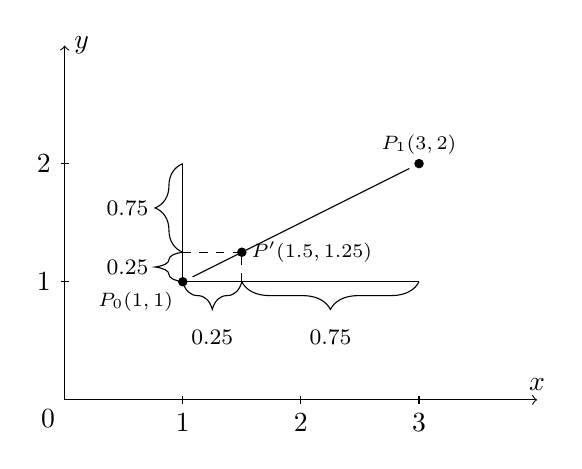
\begin{tikzpicture}[scale=1.5]
		\draw [->] (0,0) -- (0,3) node[align=left, right] {$y$};
		\draw [->] (0,0) -- (4,0) node[align=left, above] {$x$};
		\draw (0,0) node[anchor=north east,fill=white] {0};
		\foreach \x/\xtext in {1, 2, 3} 
			\draw (\x,1pt) -- (\x,-1pt) node[anchor=north,fill=white] {$\xtext$};
		\foreach \y/\ytext in {1, 2} 
			\draw (1pt,\y) -- (-1pt,\y) node[anchor=east,fill=white] {$\ytext$};
		
		\path	(1,1) node(p0) {} 
			(3,2) node(p1) {};
		\filldraw (p0) circle (1pt) node[align=center, below left] {\scriptsize $P_0(1,1)$};
		\filldraw (p1) circle (1pt) node[align=center, above] {\scriptsize $P_1(3,2)$};
		\draw (p0) -- (p1);
		\draw (1,1) -- (3,1);
		\draw (1,1) -- (1,2);
		\draw[dashed] (1.5,1) -- (1.5,1.25);
		\draw[dashed] (1,1.25) -- (1.5,1.25);
		\filldraw (1.5,1.25) circle (1pt) node[align=center, right] {\scriptsize $P'(1.5,1.25)$};
		\draw [decorate,decoration={brace,amplitude=10pt,mirror},xshift=0pt,yshift=0pt] (1,1) -- (1.5,1) node [black,midway,yshift=-20pt] {\footnotesize $0.25$};
		\draw [decorate,decoration={brace,amplitude=10pt,mirror},xshift=0pt,yshift=0pt] (1.5,1) -- (3,1) node [black,midway,yshift=-20pt] {\footnotesize $0.75$};
		
		\draw [decorate,decoration={brace,amplitude=10pt},xshift=0pt,yshift=0pt] (1,1) -- (1,1.25) node [black,midway,xshift=-20pt] {\footnotesize $0.25$};
		\draw [decorate,decoration={brace,amplitude=10pt},xshift=0pt,yshift=0pt] (1,1.25) -- (1,2) node [black,midway,xshift=-20pt] {\footnotesize $0.75$};
	\end{tikzpicture}
	\caption{Parametric linear interpolation for $t=0.25$}
\end{figure}

In the same way, as shown in Fig. 3.3, at $t=0.25$, the resulting points are one-quarter of the way between the initial and the terminal points in both axes, which is like travelling 25\% of the path since the starting point.
\end{example}

As shown in the two examples above, the $t$ value is analogous to the ratio in which the person has travelled from the initial point that a GPS device would let one know.

As such, a linear interpolation between $(x_A, y_B)$ and $(x_A,y_B)$ can be parametrically defined as following:
\begin{gather}
x(t)=x_A + (x_B - x_A)t \\
y(t)=y_A + (y_B - y_A)t
\end{gather}

At $t=0$, the interpolated point is at $(x_A, y_A)$, the initial point, and at $t=0$, it is at $(x_1,y_1)$, the terminal point. This can be considered as being at the initial point when one has travelled 0\% of the path, and as being at the terminal point when one has travelled 100\% of the path.

Parametric equations (4) and (5), however, look to be very similar. In fact, they can be combined to form a 2-dimensional (2D) vector equation. Let $P_0$ and $P_1$ be position vectors, where $P_0=(x_0,y_0)$ and $P_1=(x_1,y_1)$. Then,

\begin{equation}
P(t)=P_0 + (P_1 - P_0)t,
\end{equation}

where $P(t)$ is a function that linearly interpolates a point between $P_0$ and $P_1$ for $t \in [0,1]$. Analogously, this is a vector addition between the initial location and the path a driver has travelled so far at time $t$. Eq. (6) can be rearranged as following:

\begin{equation}
P(t)={P_0}(1-t) + {P_1}t,
\end{equation}

Eq. (7) further emphasizes the analogous nature of $t$ being the ``ratio'' \fullcite{PRAUTZ:2013} of the resulting point $P$ with respect to the initial and final points. More specifically, the ratio $t:(1-t)$ equals to the ratio of the distance from the current point $P$ with the initial point $P_0$ and the final point $P_1$, respectively, as shown in Fig. 3.4.

\begin{figure}[H]
	\centering
	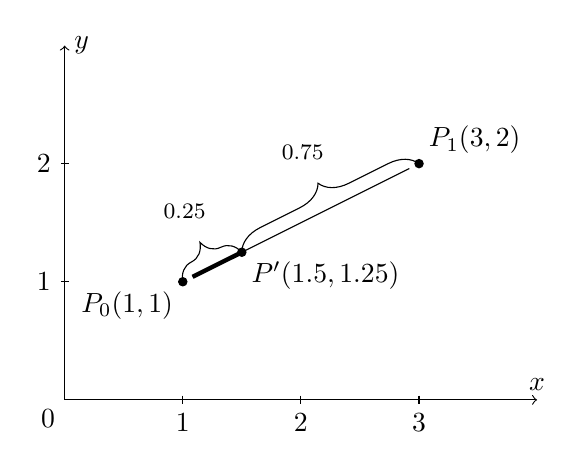
\begin{tikzpicture}[scale=1.5]
		\draw [->] (0,0) -- (0,3) node[align=left, right] {$y$};
		\draw [->] (0,0) -- (4,0) node[align=left, above] {$x$};
		\draw (0,0) node[anchor=north east,fill=white] {0};
		\foreach \x/\xtext in {1, 2, 3} 
			\draw (\x,1pt) -- (\x,-1pt) node[anchor=north,fill=white] {$\xtext$};
		\foreach \y/\ytext in {1, 2} 
			\draw (1pt,\y) -- (-1pt,\y) node[anchor=east,fill=white] {$\ytext$};
		
		\path	(1,1) node(p0) {} 
			(3,2) node(p1) {};
		\filldraw (p0) circle (1pt) node[align=center, below left] {$P_0(1,1)$};
		\filldraw (p1) circle (1pt) node[align=center, above right] {$P_1(3,2)$};
		\draw (p0) -- (p1);
		\draw[ultra thick] (p0) -- (1.5,1.25);
		\filldraw (1.5,1.25) circle (1pt) node[align=center, below right] {$P'(1.5,1.25)$};
		
		\draw [decorate,decoration={brace,amplitude=10pt},xshift=0pt,yshift=0pt] (1,1) -- (1.5,1.25) node [black,midway,yshift=20pt,xshift=-10pt] {\footnotesize $0.25$};
		\draw [decorate,decoration={brace,amplitude=10pt},xshift=0pt,yshift=0pt] (1.5,1.25) -- (3,2) node [black,midway,yshift=20pt,xshift=-10pt] {\footnotesize $0.75$};
	\end{tikzpicture}
	\caption{Ratio of $(1-t)$ and $t$ for $t=0.25$}
\end{figure}

To construct the interpolant, $t$ values with an infinitesimal interval between each other would be used. In computer systems, this would translate to having $t$ values with an interval small enough that will allow the line to appear smooth and continuous, and large enough to not harm the performance of the computer.

\section{Recursive Linear Interpolation}

Thus far, the main focus of our investigation was on the methods used to produce straight lines. However, surprisingly, linear interpolation can be repeated to produce a smooth curve. The following example will show how such can be achieved with 3 points.

\begin{example} Let $P_0 = (1,1)$, $P_1 = (2,2)$, and $P_2 = (3,1)$. By applying linear interpolation, we know that we can produce straight lines between these three points using the vector equation $P(t) = P_A(1-t) + P_{B}t$. This is shown in Fig. 4.1.

\begin{figure}[H]
	\centering
	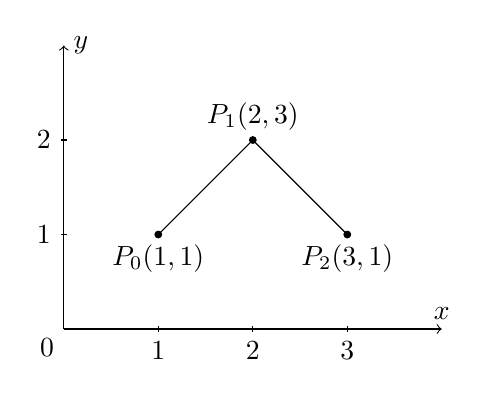
\begin{tikzpicture}[scale=1.2]
		\draw [->] (0,0) -- (0,3) node[align=left, right] {$y$};
		\draw [->] (0,0) -- (4,0) node[align=left, above] {$x$};
		\draw (0,0) node[anchor=north east,fill=white] {0};
		\foreach \x/\xtext in {1, 2, 3} 
			\draw (\x,1pt) -- (\x,-1pt) node[anchor=north,fill=white] {$\xtext$};
		\foreach \y/\ytext in {1, 2} 
			\draw (1pt,\y) -- (-1pt,\y) node[anchor=east,fill=white] {$\ytext$};
		
		\filldraw (1,1) circle (1pt) node[align=center, below] {$P_0(1,1)$};
		\filldraw (2,2) circle (1pt) node[align=center, above] {$P_1(2,3)$};
		\filldraw (3,1) circle (1pt) node[align=center, below] {$P_2(3,1)$};
		
		\draw (1,1) -- (2,2) -- (3,1);
	\end{tikzpicture}
	\caption{Linear interpolants between $P_0$ and $P_1$, and $P_1$ and $P_2$}
\end{figure}

Let $P_{0 \dotsc 1}$ be a linearly interpolated point between $P_0$ and $P_1$ at $t=0.5$. Similarly, let $P_{1 \dotsc 2}$ be the linearly interpolated point between $P_1$ and $P_2$ at $t=0.5$. These newly interpolated points can be used as the starting and terminal points of new linear interpolation, as shown in Fig. 4.2.

\begin{figure}[H]
	\centering
	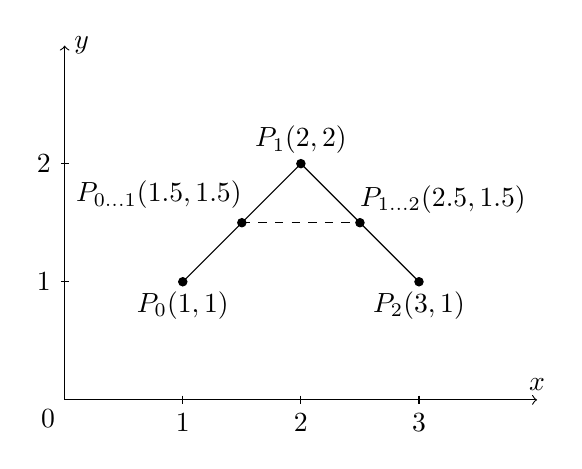
\begin{tikzpicture}[scale=1.5]
%	\begin{scriptsize}
		\draw [->] (0,0) -- (0,3) node[align=left, right] {$y$};
		\draw [->] (0,0) -- (4,0) node[align=left, above] {$x$};
		\draw (0,0) node[anchor=north east,fill=white] {0};
		\foreach \x/\xtext in {1, 2, 3} 
			\draw (\x,1pt) -- (\x,-1pt) node[anchor=north,fill=white] {$\xtext$};
		\foreach \y/\ytext in {1, 2} 
			\draw (1pt,\y) -- (-1pt,\y) node[anchor=east,fill=white] {$\ytext$};
		
		\filldraw (1,1) circle (1pt) node[align=center, below] {$P_0(1,1)$};
		\filldraw (2,2) circle (1pt) node[align=center, above] {$P_1(2,2)$};
		\filldraw (3,1) circle (1pt) node[align=center, below] {$P_2(3,1)$};
		
		\draw (1,1) -- (2,2) -- (3,1);
		
		\filldraw (1.5,1.5) circle (1pt) node[align=center, xshift=-30pt, yshift=10pt] {$P_{0 \dotsc 1}(1.5,1.5)$};
		\filldraw (2.5,1.5) circle (1pt) node[align=center, xshift=30pt, above] {$P_{1 \dotsc 2}(2.5,1.5)$};
		\draw[dashed] (1.5,1.5) -- (2.5,1.5);
%	\end{scriptsize}
	\end{tikzpicture}
	\caption{Linear interpolant of $P_{0 \dotsc 1}$ and $P_{1 \dotsc 2}$}
\end{figure}

Finally, let $P_{0 \dotsc 2}$ be the linearly interpolated point between $P_{0 \dotsc 1}$ and $P_{1 \dotsc 2}$. $P_{0 \dotsc 2}$, then, is a resulting point of the quadratic interpolation from points $P_0$, $P_1$, and $P_2$ at $t=0.5$, as shown in Fig. 4.3.

\begin{figure}[H]
	\centering
	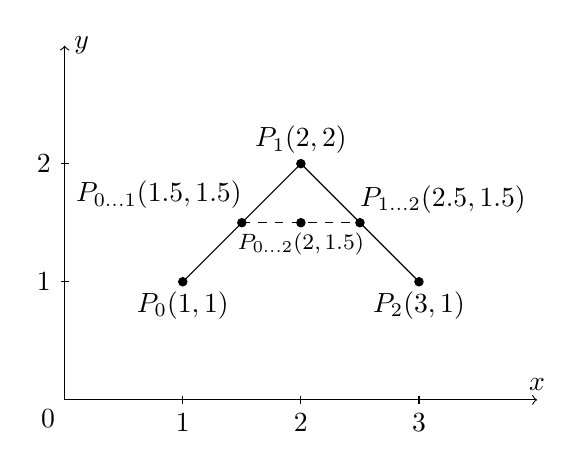
\begin{tikzpicture}[scale=1.5]
%	\begin{scriptsize}
		\draw [->] (0,0) -- (0,3) node[align=left, right] {$y$};
		\draw [->] (0,0) -- (4,0) node[align=left, above] {$x$};
		\draw (0,0) node[anchor=north east,fill=white] {0};
		\foreach \x/\xtext in {1, 2, 3} 
			\draw (\x,1pt) -- (\x,-1pt) node[anchor=north,fill=white] {$\xtext$};
		\foreach \y/\ytext in {1, 2} 
			\draw (1pt,\y) -- (-1pt,\y) node[anchor=east,fill=white] {$\ytext$};
		
		\filldraw (1,1) circle (1pt) node[align=center, below] {$P_0(1,1)$};
		\filldraw (2,2) circle (1pt) node[align=center, above] {$P_1(2,2)$};
		\filldraw (3,1) circle (1pt) node[align=center, below] {$P_2(3,1)$};
		
		\draw (1,1) -- (2,2) -- (3,1);
		
		\filldraw (1.5,1.5) circle (1pt) node[align=center, xshift=-30pt, yshift=10pt] {$P_{0 \dotsc 1}(1.5,1.5)$};
		\filldraw (2.5,1.5) circle (1pt) node[align=center, xshift=30pt, above] {$P_{1 \dotsc 2}(2.5,1.5)$};
		\draw[dashed] (1.5,1.5) -- (2.5,1.5);
		
		\filldraw (2,1.5) circle (1pt) node[align=center, xshift=0pt, below] {\footnotesize $P_{0 \dotsc 2}(2,1.5)$};
%	\end{scriptsize}
	\end{tikzpicture}
	\caption{Quadratic interpolation at $t=0.5$}
\end{figure}

This technique of repeated linear interpolation can be performed at $t=0.25$ and $t=0.75$, as shown in Fig. 4.4 and 4.5.

\begin{figure}[H]
	\centering
	\begin{minipage}{.5\textwidth}
	\centering
	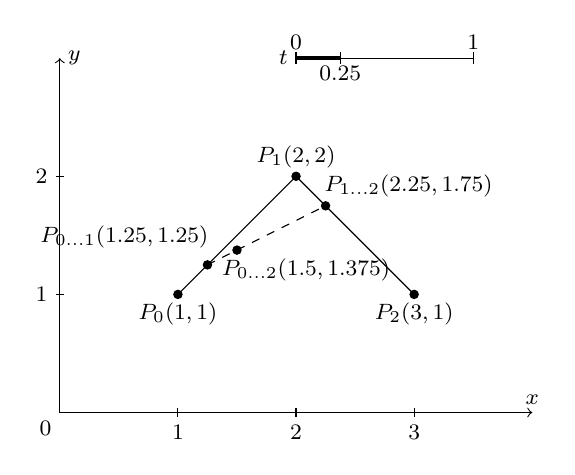
\begin{tikzpicture}[scale=1.5]
	\begin{footnotesize}
		\draw (2,3) -- (3.5, 3) node[pos=0, left]{$t$} node[pos=0, above]{0} node[pos=0.25, below]{0.25} node[pos=1, above]{1};
		\draw[ultra thick] (2,3) -- (2.375, 3);
		\draw (2,3-0.05) -- (2,3+0.05);
		\draw (2.375,3-0.05) -- (2.375,3+0.05);
		\draw (3.5,3-0.05) -- (3.5,3+0.05);
		
		\draw [->] (0,0) -- (0,3) node[align=left, right] {$y$};
		\draw [->] (0,0) -- (4,0) node[align=left, above] {$x$};
		\draw (0,0) node[anchor=north east,fill=white] {0};
		\foreach \x/\xtext in {1, 2, 3} 
			\draw (\x,1pt) -- (\x,-1pt) node[anchor=north,fill=white] {$\xtext$};
		\foreach \y/\ytext in {1, 2} 
			\draw (1pt,\y) -- (-1pt,\y) node[anchor=east,fill=white] {$\ytext$};
		
		\filldraw (1,1) circle (1pt) node[align=center, below] {$P_0(1,1)$};
		\filldraw (2,2) circle (1pt) node[align=center, above] {$P_1(2,2)$};
		\filldraw (3,1) circle (1pt) node[align=center, below] {$P_2(3,1)$};
		
		\draw (1,1) -- (2,2) -- (3,1);
		
		\filldraw (1.25,1.25) circle (1pt) node[align=center, xshift=-30pt, yshift=10pt] {$P_{0 \dotsc 1}(1.25,1.25)$};
		\filldraw (2.25,1.75) circle (1pt) node[align=center, xshift=30pt, above] {$P_{1 \dotsc 2}(2.25,1.75)$};
		\draw[dashed] (1.25,1.25) -- (2.25,1.75);
		
		\filldraw (1.5,1.375) circle (1pt) node[align=center, xshift=25pt, below] { $P_{0 \dotsc 2}(1.5,1.375)$};
	\end{footnotesize}
	\end{tikzpicture}
	\captionof{figure}{\small Quadratic interpolation at $t=0.25$}
	\end{minipage}%
	\begin{minipage}{.5\textwidth}
    		\centering
    		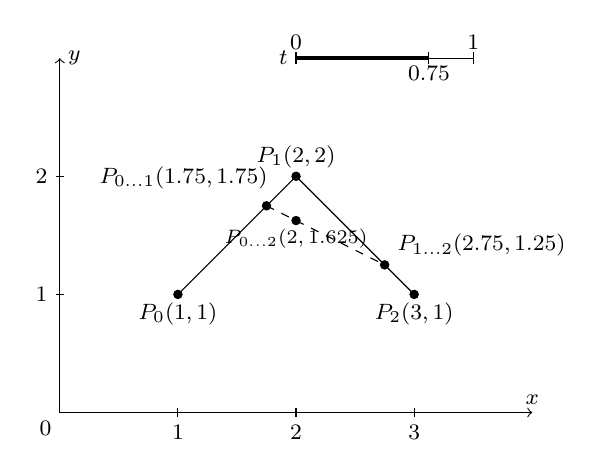
\begin{tikzpicture}[scale=1.5]
    		\begin{footnotesize}
    			\draw (2,3) -- (3.5, 3) node[pos=0, left]{$t$} node[pos=0, above]{0} node[pos=0.75, below]{0.75} node[pos=1, above]{1};
	    		\draw[ultra thick] (2,3) -- (3.125, 3);
	    		\draw (2,3-0.05) -- (2,3+0.05);
	    		\draw (3.125,3-0.05) -- (3.125,3+0.05);
	    		\draw (3.5,3-0.05) -- (3.5,3+0.05);
    		
	    		\draw [->] (0,0) -- (0,3) node[align=left, right] {$y$};
	    		\draw [->] (0,0) -- (4,0) node[align=left, above] {$x$};
	    		\draw (0,0) node[anchor=north east,fill=white] {0};
	    		\foreach \x/\xtext in {1, 2, 3} 
    			\draw (\x,1pt) -- (\x,-1pt) node[anchor=north,fill=white] {$\xtext$};
	    		\foreach \y/\ytext in {1, 2} 
	    			\draw (1pt,\y) -- (-1pt,\y) node[anchor=east,fill=white] {$\ytext$};
	    		
	    		\filldraw (1,1) circle (1pt) node[align=center, below] {$P_0(1,1)$};
	    		\filldraw (2,2) circle (1pt) node[align=center, above] {$P_1(2,2)$};
	    		\filldraw (3,1) circle (1pt) node[align=center, below] {$P_2(3,1)$};
	    		
	    		\draw (1,1) -- (2,2) -- (3,1);
	    		
	    		\filldraw (1.75,1.75) circle (1pt) node[align=center, xshift=-30pt, yshift=10pt] {$P_{0 \dotsc 1}(1.75,1.75)$};
	    		\filldraw (2.75,1.25) circle (1pt) node[align=center, xshift=35pt, above] {$P_{1 \dotsc 2}(2.75,1.25)$};
	    		\draw[dashed] (1.75,1.75) -- (2.75,1.25);
	    		
	    		\filldraw (2,1.625) circle (1pt) node[align=center, below] {\scriptsize $P_{0 \dotsc 2}(2,1.625)$};
	    	\end{footnotesize}
	    	\end{tikzpicture}
	    	\captionof{figure}{\small Quadratic interpolation at $t=0.75$}
	\end{minipage}
\end{figure}

\end{example}

At $t=0$ and $t=1$, the quadratic interpolation always yields points identical to the first and last of the original point, respectively.

\begin{example} The points $P_0$, $P_1$ and $P_2$ are defined as that of example 4.1. At $t=0$, the two linearly interpolated points are

\begin{equation_nogap}\begin{aligned}
P_{0 \dotsc 1}(0)	& = P_0(1-0) + P_1(0) \\
			& = P_0.\\
P_{1 \dotsc 2}(0)	& = P_1(1-0) + P_2(0) \\
			& = P_1. \\
			\\
\end{aligned}\end{equation_nogap}

Then, the resulting point from the quadratic interpolation is

\begin{equation_nogap}\begin{aligned}
P_{0 \dotsc 2}(0)	& = P_{0 \dotsc 1}(1-0) + P_{1 \dotsc 2}(0) \\
			& = P_{0 \dotsc 1} \\
			& = P_0, \\
			\\
\end{aligned}\end{equation_nogap}

which is the first of the original points, $P_0$.
\end{example}

\begin{example} Given the same three points as Examples 4.1 and 4.2, at $t=1$, the two linearly interpolated points are

\begin{equation_nogap}\begin{aligned}
P_{0 \dotsc 1}(1)	& = P_0(1-1) + P_1(1) \\
			& = P_1.\\
P_{1 \dotsc 2}(1)	& = P_1(1-1) + P_2(1) \\
			& = P_2. \\
			\\
\end{aligned}\end{equation_nogap}

Then, the resulting point from the quadratic interpolation is

\begin{equation_nogap}\begin{aligned}
P_{0 \dotsc 2}(1)	& = P_{0 \dotsc 1}(1-1) + P_{1 \dotsc 2}(1) \\
			& = P_{1 \dotsc 2} \\
			& = P_2, \\
\\
\end{aligned}\end{equation_nogap}

which is the last of the original points, $P_2$.
\end{example}

With infinitesimal interval of $t$ values, the quadratic interpolant can be consturcted, as shown in Fig. 4.6. In computer systems, this would translate to having small enough interval of $t$ value that will allow the curve to look smooth, and also one that is large enough that will not harm the computer's performance with redundant calculations.

\begin{figure}[H]
	\centering
	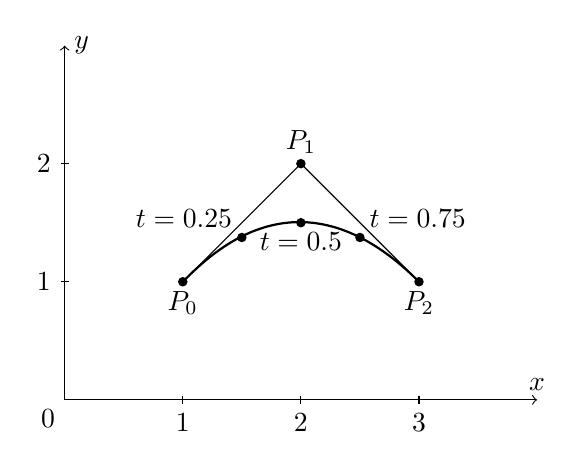
\begin{tikzpicture}[scale=1.5]
		\draw [->] (0,0) -- (0,3) node[align=left, right] {$y$};
		\draw [->] (0,0) -- (4,0) node[align=left, above] {$x$};
		\draw (0,0) node[anchor=north east,fill=white] {0};
		\foreach \x/\xtext in {1, 2, 3} 
			\draw (\x,1pt) -- (\x,-1pt) node[anchor=north,fill=white] {$\xtext$};
		\foreach \y/\ytext in {1, 2} 
			\draw (1pt,\y) -- (-1pt,\y) node[anchor=east,fill=white] {$\ytext$};
		
		\filldraw (1,1) circle (1pt) node[align=center, below] {$P_0$};
		\filldraw (2,2) circle (1pt) node[align=center, above] {$P_1$};
		\filldraw (3,1) circle (1pt) node[align=center, below] {$P_2$};
		
		\draw (1,1) -- (2,2) -- (3,1);
		
		\filldraw (2,1.5) circle (1pt) node[align=center, below] {$t=0.5$};
		\filldraw (1.5,1.375) circle (1pt) node[align=center, above left] {$t=0.25$};
		\filldraw (2.5,1.375) circle (1pt) node[align=center, above right] {$t=0.75$};
		
		\draw[thick] (1,1) .. controls (1.25,1.25) and (2,2) .. (3,1);
	\end{tikzpicture}
	\caption{Quadratic interpolant}
\end{figure}

This repeated linear interpolation is called the \textbf{De Casteljau construction}, or the \textbf{De Casteljau algorithm} \cite{DECAST:1959}. Because this algorithm repeats itself by producing new interpolation from previously interpolated points, it is described as being "recursive" \cite{PRAUTZ:2013}, meaning that it repeats itself to meet the objective. The curve produced from this construction is later formalized and popularized by Pierre B\'ezier \fullcite{FARIN:2001}, by whom this curve, the \textbf{B\'ezier curve}, was named after.

In the De Casteljau algorithm, the only information needed to construct any curve is the initial points, such as $P_0, P_1$ and $P_2$ shown in Fig. 4.6. As such, they are the ones that controls the appearance of the resulting curve. Hence, these points are referred to as the \textbf{control points} of the B\'ezier curve \cite{PRAUTZ:2013}.

Thus far, we have investigated on construction of quadratic curves with three B\'ezier control points. However, by following the similar process of repeating linear interpolation, curves with higher number of control points can be easily constructed, as shown in the following example.

\begin{example} Let $P_0 = (1, 1), P_1 = (1, 5), P_2 = (5, 5),$ and $P_3 = (5, 1)$. With linear interpolation performed for each consecutive pairs of control points, a set of straight interpolants can be produced as shown in Fig. 4.7.

\begin{figure}[H]
	\centering
	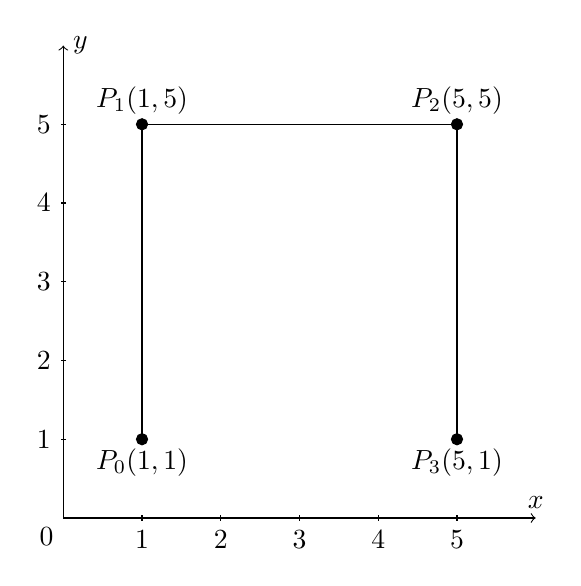
\begin{tikzpicture}[scale=1]
		\coordinate (P_0) at (1, 1);
		\coordinate (P_1) at (1, 5);
		\coordinate (P_2) at (5, 5);
		\coordinate (P_3) at (5, 1);
		
		\draw [->] (0,0) -- (0,6) node[align=left, right] {$y$};
		\draw [->] (0,0) -- (6,0) node[align=left, above] {$x$};
		\draw (0,0) node[anchor=north east,fill=white] {0};
		\foreach \x/\xtext in {1, 2, 3, 4, 5} 
			\draw (\x,1pt) -- (\x,-1pt) node[anchor=north,fill=white] {$\xtext$};
		\foreach \y/\ytext in {1, 2, 3, 4, 5} 
			\draw (1pt,\y) -- (-1pt,\y) node[anchor=east,fill=white] {$\ytext$};
		
		\draw (P_0) -- (P_1) -- (P_2) -- (P_3);
		
		\filldraw (P_0) circle (2pt) node[align=center, below] {$P_0(1,1)$};
		\filldraw (P_1) circle (2pt) node[align=center, above] {$P_1(1,5)$};
		\filldraw (P_2) circle (2pt) node[align=center, above] {$P_2(5,5)$};
		\filldraw (P_3) circle (2pt) node[align=center, below] {$P_3(5,1)$};
	\end{tikzpicture}
	\caption{Linear interpolants between the four B\'ezier control points}
\end{figure}

In order to produce an interpolated point using the control points, the points $P_{0 \dotsc 1}, P_{1 \dotsc 2}$ and $P_{2 \dotsc 3}$ must be interpolated first. These points can be used to perform another set of linear interpolations, as shown in Fig. 4.8.

\begin{figure}[H]
	\centering
	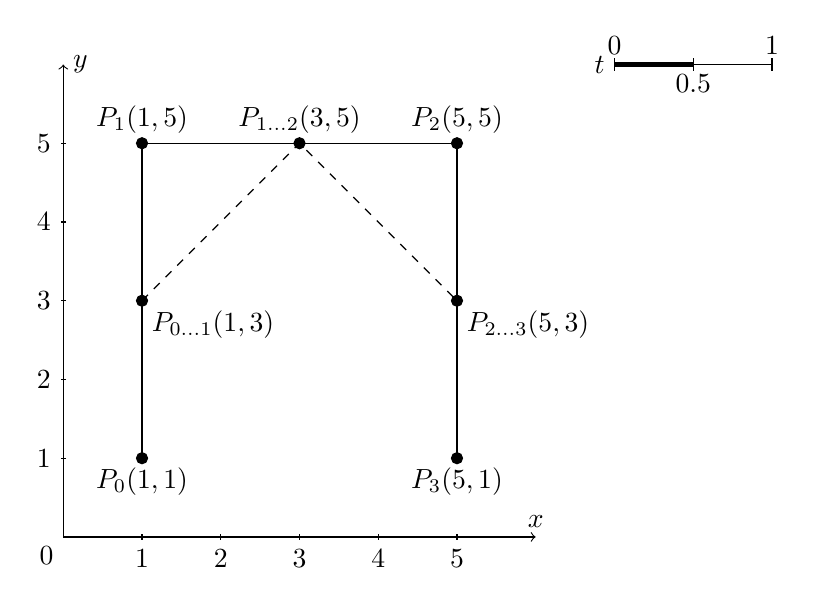
\begin{tikzpicture}[scale=1]
		% Coordinates
		\coordinate (P_0) at (1, 1);
		\coordinate (P_1) at (1, 5);
		\coordinate (P_2) at (5, 5);
		\coordinate (P_3) at (5, 1);
		
		\coordinate (P_0-1) at (1, 3);
		\coordinate (P_1-2) at (3, 5);
		\coordinate (P_2-3) at (5, 3);
		
		% Draw X and Y axes
		\draw [->] (0,0) -- (0,6) node[align=left, right] {$y$};
		\draw [->] (0,0) -- (6,0) node[align=left, above] {$x$};
		\draw (0,0) node[anchor=north east,fill=white] {0};
		\foreach \x/\xtext in {1, 2, 3, 4, 5} 
			\draw (\x,1pt) -- (\x,-1pt) node[anchor=north,fill=white] {$\xtext$};
		\foreach \y/\ytext in {1, 2, 3, 4, 5} 
			\draw (1pt,\y) -- (-1pt,\y) node[anchor=east,fill=white] {$\ytext$};
			
		% Draw t line
		\draw (7,6) -- (9, 6) node[pos=0, left]{$t$} node[pos=0, above]{0} node[pos=0.5, below]{0.5} node[pos=1, above]{1};
	    	\foreach \t/\ttext in {7, 8, 9}
			\draw (\t, 6+0.08) -- (\t, 6-0.08);
		\draw[ultra thick] (7, 6) -- (8, 6);
		
		% First interpolation
		\draw (P_0) -- (P_1) -- (P_2) -- (P_3);
		
		\filldraw (P_0) circle (2pt) node[align=center, below] {$P_0(1,1)$};
		\filldraw (P_1) circle (2pt) node[align=center, above] {$P_1(1,5)$};
		\filldraw (P_2) circle (2pt) node[align=center, above] {$P_2(5,5)$};
		\filldraw (P_3) circle (2pt) node[align=center, below] {$P_3(5,1)$};
		
		% Second Interpolation
		\draw[dashed] (P_0-1) -- (P_1-2) -- (P_2-3);
		
		\filldraw (P_0-1) circle (2pt) node[align=center, below right] {$P_{0 \dotsc 1}(1,3)$};
		\filldraw (P_1-2) circle (2pt) node[align=center, above] {$P_{1 \dotsc 2}(3,5)$};
		\filldraw (P_2-3) circle (2pt) node[align=center, below right] {$P_{2 \dotsc 3}(5,3)$};
	\end{tikzpicture}
	\caption{Second recursion of De Casteljau algorithm}
\end{figure}

Then, the points $P_{0 \dotsc 1}, P_{1 \dotsc 2}$ and $P_{2 \dotsc 3}$ can be used to perform another linear interpolation, as shown in Fig. 4.9.

\begin{figure}[H]
	\centering
	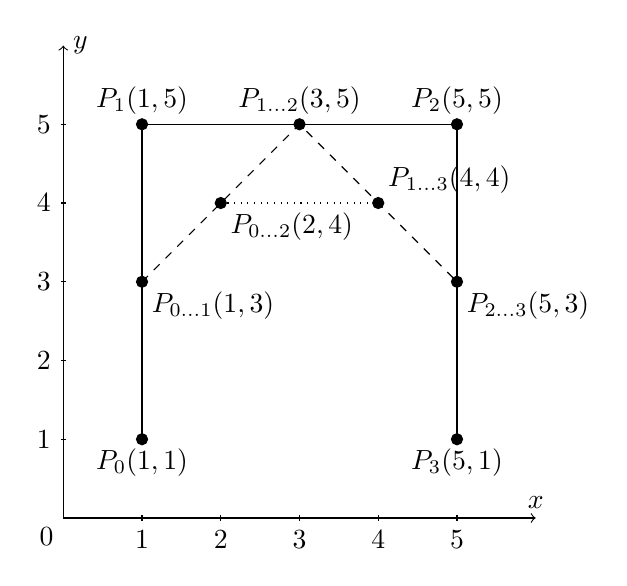
\begin{tikzpicture}[scale=1]
		% Coordinates
		\coordinate (P_0) at (1, 1);
		\coordinate (P_1) at (1, 5);
		\coordinate (P_2) at (5, 5);
		\coordinate (P_3) at (5, 1);
		
		\coordinate (P_0-1) at (1, 3);
		\coordinate (P_1-2) at (3, 5);
		\coordinate (P_2-3) at (5, 3);
		
		\coordinate (P_0-2) at (2, 4);
		\coordinate (P_1-3) at (4, 4);
		
		% Draw X and Y axes
		\draw [->] (0,0) -- (0,6) node[align=left, right] {$y$};
		\draw [->] (0,0) -- (6,0) node[align=left, above] {$x$};
		\draw (0,0) node[anchor=north east,fill=white] {0};
		\foreach \x/\xtext in {1, 2, 3, 4, 5} 
			\draw (\x,1pt) -- (\x,-1pt) node[anchor=north,fill=white] {$\xtext$};
		\foreach \y/\ytext in {1, 2, 3, 4, 5} 
			\draw (1pt,\y) -- (-1pt,\y) node[anchor=east,fill=white] {$\ytext$};
			
		% First interpolation
		\draw (P_0) -- (P_1) -- (P_2) -- (P_3);
		
		\filldraw (P_0) circle (2pt) node[align=center, below] {$P_0(1,1)$};
		\filldraw (P_1) circle (2pt) node[align=center, above] {$P_1(1,5)$};
		\filldraw (P_2) circle (2pt) node[align=center, above] {$P_2(5,5)$};
		\filldraw (P_3) circle (2pt) node[align=center, below] {$P_3(5,1)$};
		
		% Second Interpolation
		\draw[dashed] (P_0-1) -- (P_1-2) -- (P_2-3);
		
		\filldraw (P_0-1) circle (2pt) node[align=center, below right] {$P_{0 \dotsc 1}(1,3)$};
		\filldraw (P_1-2) circle (2pt) node[align=center, above] {$P_{1 \dotsc 2}(3,5)$};
		\filldraw (P_2-3) circle (2pt) node[align=center, below right] {$P_{2 \dotsc 3}(5,3)$};
		
		% Third Interpolation
		\draw[dotted] (P_0-2) -- (P_1-3);
		
		\filldraw (P_0-2) circle (2pt) node[align=center, below right] {$P_{0 \dotsc 2}(2,4)$};
		\filldraw (P_1-3) circle (2pt) node[align=center, above right] {$P_{1 \dotsc 3}(4,4)$};
	\end{tikzpicture}
	\caption{Third recursion of De Casteljau algorithm}
\end{figure}

Finally, the resulting point, $P_{0 \dotsc 3}$, of the cubic interpolation at $t=0.5$ is obtained using the points $P_{0 \dotsc 2}$ and $P_{1 \dotsc 3}$, as shown in Fig. 4.10:

\begin{figure}[H]
	\centering
	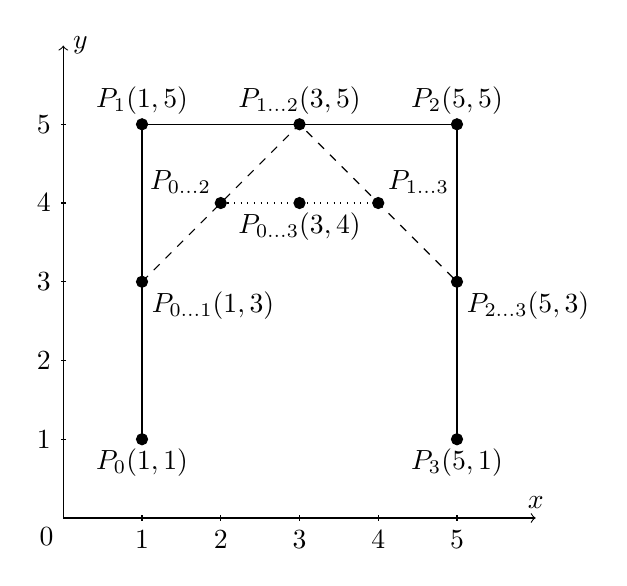
\begin{tikzpicture}[scale=1]
		% Coordinates
		\coordinate (P_0) at (1, 1);
		\coordinate (P_1) at (1, 5);
		\coordinate (P_2) at (5, 5);
		\coordinate (P_3) at (5, 1);
		
		\coordinate (P_0-1) at (1, 3);
		\coordinate (P_1-2) at (3, 5);
		\coordinate (P_2-3) at (5, 3);
		
		\coordinate (P_0-2) at (2, 4);
		\coordinate (P_1-3) at (4, 4);
		
		\coordinate (P_0-3) at (3, 4);
		
		% Draw X and Y axes
		\draw [->] (0,0) -- (0,6) node[align=left, right] {$y$};
		\draw [->] (0,0) -- (6,0) node[align=left, above] {$x$};
		\draw (0,0) node[anchor=north east,fill=white] {0};
		\foreach \x/\xtext in {1, 2, 3, 4, 5} 
			\draw (\x,1pt) -- (\x,-1pt) node[anchor=north,fill=white] {$\xtext$};
		\foreach \y/\ytext in {1, 2, 3, 4, 5} 
			\draw (1pt,\y) -- (-1pt,\y) node[anchor=east,fill=white] {$\ytext$};
			
		% First interpolation
		\draw (P_0) -- (P_1) -- (P_2) -- (P_3);
		
		\filldraw (P_0) circle (2pt) node[align=center, below] {$P_0(1,1)$};
		\filldraw (P_1) circle (2pt) node[align=center, above] {$P_1(1,5)$};
		\filldraw (P_2) circle (2pt) node[align=center, above] {$P_2(5,5)$};
		\filldraw (P_3) circle (2pt) node[align=center, below] {$P_3(5,1)$};
		
		% Second Interpolation
		\draw[dashed] (P_0-1) -- (P_1-2) -- (P_2-3);
		
		\filldraw (P_0-1) circle (2pt) node[align=center, below right] {$P_{0 \dotsc 1}(1,3)$};
		\filldraw (P_1-2) circle (2pt) node[align=center, above] {$P_{1 \dotsc 2}(3,5)$};
		\filldraw (P_2-3) circle (2pt) node[align=center, below right] {$P_{2 \dotsc 3}(5,3)$};
		
		% Third Interpolation
		\draw[dotted] (P_0-2) -- (P_1-3);
		
		\filldraw (P_0-2) circle (2pt) node[align=center, above left] {$P_{0 \dotsc 2}$};
		\filldraw (P_1-3) circle (2pt) node[align=center, above right] {$P_{1 \dotsc 3}$};
		
		% Interpolated Point
		\filldraw (P_0-3) circle (2pt) node[align=center, below] {$P_{0 \dotsc 3}(3, 4) $};
	\end{tikzpicture}
	\caption{Resulting point of the cubic interpolation}
\end{figure}

\end{example}

As such, the De Casteljau algorithm can be expressed as the following set of procedure:

\begin{enumerate}
\item Interpolate a set of points at $t \in [0, 1]$ for each of the consecutive pair of control points.
\item Repeat step \#1 with newly interpolated points, until a single point is left.
\end{enumerate}

Thus far, the B\'ezier curve has vaguely been mentioned, and its mathematical definition is yet unclear. However, this algorithm can be used to deduce the formal definition of a B\'ezier curve. Let $P_{a \dotsc b}(t)$ be a function that gives an interpolated point from a set of control points $P_a, P_{a+1}, P_{a+2},  \dotsc  , P_{b-1}, P_b$, where $a, b \in \mathbb Z_{\geq 0}$ and $a \geq b$. If $a = b$, $P_{a \dotsc b}(t) = P_a = P_b$. Next, let the control points of a B\'ezier curve be $P_0, P_1, P_2,  \dotsc  , P_{n-1}, P_{n}$. Performing a set of linear interpolation to consecutive pairs of control points at $t$ gives the following:

\begin{equation_nogap}\begin{aligned}
P_{0 \dotsc 1}(t)	& = P_0(1-t) + P_1t, \\
P_{1 \dotsc 2}(t)	& = P_1(1-t) + P_2t, \\
P_{2 \dotsc 3}(t)	& = P_2(1-t) + P_3t, \\
& \vdotswithin{=} \notag \\
P_{n-1 \dotsc n}(t)	& = P_{n-1}(1-t) + P_nt. \\
\\
\end{aligned}\end{equation_nogap}

The newly interpolated points can than be used to perform another set of interpolation.

\begin{equation_nogap}\begin{aligned}
P_{0 \dotsc 2}(t)	& = [P_{0 \dotsc 1}(t)](1-t) + [P_{1 \dotsc 2}(t)]t, \\
P_{1 \dotsc 3}(t)	& = [P_{1 \dotsc 2}(t)](1-t) + [P_{2 \dotsc 3}(t)]t, \\
P_{2 \dotsc 4}(t)	& = [P_{2 \dotsc 3}(t)](1-t) + [P_{3 \dotsc 4}(t)]t, \\
& \vdotswithin{=} \notag \\
P_{n-2 \dotsc n}(t)	& = [P_{n-2 \dotsc n-1}(t)](1-t) + [P_{n-1 \dotsc n}(t)]t. \\
\\
\end{aligned}\end{equation_nogap}

Substituting the interpolation functions with their definitions,

\begin{equation_nogap}\begin{aligned}
P_{0 \dotsc 2}(t)	& = [P_0(1-t)+P_1t](1-t) + [P_1(1-t)+P_2t]t, \\
P_{1 \dotsc 3}(t)	& = [P_1(1-t)+P_2t](1-t) + [P_2(1-t)+P_3t]t, \\
P_{2 \dotsc 4}(t)	& = [P_2(1-t)+P_3t](1-t) + [P_3(1-t)+P_4t]t, \\
& \vdotswithin{=} \notag \\
P_{n-2 \dotsc n}(t)	& = [P_{n-2}(1-t)+P_{n-1}t](1-t) + [P_{n-1}(1-t)+P_nt]t. \\
\\
\end{aligned}\end{equation_nogap}

Simplifying the equations above,

\begin{equation_nogap}\begin{aligned}
P_{0 \dotsc 2}(t)	& = P_0(1-t)^2 + 2P_1(1-t)t + P_2t^2, \\
P_{1 \dotsc 3}(t)	& = P_1(1-t)^2 + 2P_2(1-t)t + P_3t^2, \\
P_{2 \dotsc 4}(t)	& = P_2(1-t)^2 + 2P_3(1-t)t + P_4t^2, \\
& \vdotswithin{=} \notag \\
P_{n-2 \dotsc n}(t)	& = P_{n-2}(1-t)^2 + 2P_{n-1}(1-t)t + P_{n}t^2. \\
\\
\end{aligned}\end{equation_nogap}

\begin{absnopagebreak}
Following the same procedure of interpolating and simplifying yields the following:

\begin{equation_nogap}\begin{aligned}
P_{0 \dotsc 3}(t)	& = P_0(1-t)^3 + 3P_1(1-t)^2t + 3P_2(1-t)t^2 + P_3t^3, \\
P_{1 \dotsc 4}(t)	& = P_1(1-t)^3 + 3P_2(1-t)^2t + 3P_3(1-t)t^2 + P_4t^3, \\
P_{2 \dotsc 5}(t)	& = P_2(1-t)^3 + 3P_3(1-t)^2t + 3P_4(1-t)t^2 + P_5t^3, \\
& \vdotswithin{=} \notag \\
P_{n-3 \dotsc n}(t)	& = P_{n-3}(1-t)^3 + 3P_{n-2}(1-t)^2t + 3P_{n-1}(1-t)t^2 + P_{n}t^3. \\
\\
\end{aligned}\end{equation_nogap}
\end{absnopagebreak}

Repeating the same procedure again,

\begin{equation_nogap}\begin{aligned}
P_{0 \dotsc 4}(t)	& = P_0(1-t)^4 + 4P_1(1-t)^3t + 6P_2(1-t)^2t^2 + 4P_3(1-t)t^3 + P_4t^4, \\
P_{1 \dotsc 5}(t)	& = P_1(1-t)^4 + 4P_2(1-t)^3t + 6P_3(1-t)^2t^2 + 4P_4(1-t)t^3 + P_5t^4, \\
P_{2 \dotsc 6}(t)	& = P_2(1-t)^4 + 4P_3(1-t)^3t + 6P_4(1-t)^2t^2 + 4P_5(1-t)t^3 + P_6t^4, \\
& \vdotswithin{=} \notag \\
P_{n-4 \dotsc n}(t)	& = P_{n-4}(1-t)^4 + 4P_{n-3}(1-t)^3t + 6P_{n-2}(1-t)^2t^2 + 4P_{n-1}(1-t)t^3 + P_{n}t^4. \\
\\
\end{aligned}\end{equation_nogap}

A pattern that imitates binomial expansion of $((1-t) + t)^n$ emerges, along with the control points multiplied as coefficients of each terms. Continuing on a similar manner, the complete equation of interpolated B\'ezier curve is obtained.

\begin{multline}
P_{0 \dotsc n}(t) = 	P_0 \binom{n}{0}(1-t)^n + P_1 \binom{n}{1}(1-t)^{n-1}t + P_2 \binom{n}{2}(1-t)^{n-2}t^2 \\
				+ \dotsb + P_k \binom{n}{k}(1-t)^{n-k}t^k + \dotsb + P_{n-1} \binom{n}{n-1}(1-t)t^{n-1} + P_n \binom{n}{n}t^n,
\end{multline}

where $\binom{n}{k}$ is a binomial coefficient ($\binom{n}{k} = \frac{n!}{k!(n-k)!}$). Rewriting the equation above,

\begin{equation}
P_{0 \dotsc n}(t) = \sum_{i=0}^{n} {P_i \binom{n}{i} (1-t)^{n-1} t^i}.
\end{equation}

This, in fact, is the definition of the B\'ezier curve, which is written as $b_n(t)$ for curves with $n+1$ control points. As such, the mathematical development of B\'ezier curves from simple linear interpolation has been investigated so far. The following part of the essay will examine the properties of B\'eizer curves and why they allow is to be one of the most favoured method of describing curves in computer systems.

\newpage

\bibliographystyle{apacite}
\bibliography{ee_bibliography}

\end{document}  